
    




    
\documentclass[oneside,final,12pt]{extreport}

    
    \usepackage[breakable]{tcolorbox}
    \tcbset{nobeforeafter} % prevents tcolorboxes being placing in paragraphs
    \usepackage{float}
    \floatplacement{figure}{H} % forces figures to be placed at the correct location
    
    \usepackage[T1]{fontenc}
    % Nicer default font (+ math font) than Computer Modern for most use cases
    \usepackage{mathpazo}

    % Basic figure setup, for now with no caption control since it's done
    % automatically by Pandoc (which extracts ![](path) syntax from Markdown).
    \usepackage{graphicx}
    % We will generate all images so they have a width \maxwidth. This means
    % that they will get their normal width if they fit onto the page, but
    % are scaled down if they would overflow the margins.
    \makeatletter
    \def\maxwidth{\ifdim\Gin@nat@width>\linewidth\linewidth
    \else\Gin@nat@width\fi}
    \makeatother
    \let\Oldincludegraphics\includegraphics
    % Set max figure width to be 80% of text width, for now hardcoded.
    \renewcommand{\includegraphics}[1]{\Oldincludegraphics[width=.8\maxwidth]{#1}}
    % Ensure that by default, figures have no caption (until we provide a
    % proper Figure object with a Caption API and a way to capture that
    % in the conversion process - todo).
    \usepackage{caption}
    \DeclareCaptionLabelFormat{nolabel}{}
    \captionsetup{labelformat=nolabel}

    \usepackage{adjustbox} % Used to constrain images to a maximum size 
    \usepackage{xcolor} % Allow colors to be defined
    \usepackage{enumerate} % Needed for markdown enumerations to work
    \usepackage{amsmath} % Equations
    \usepackage{amssymb} % Equations
    \usepackage{textcomp} % defines textquotesingle
    % Hack from http://tex.stackexchange.com/a/47451/13684:
    \AtBeginDocument{%
        \def\PYZsq{\textquotesingle}% Upright quotes in Pygmentized code
    }
    \usepackage{upquote} % Upright quotes for verbatim code
    \usepackage{eurosym} % defines \euro
    \usepackage[mathletters]{ucs} % Extended unicode (utf-8) support
    \usepackage[utf8x]{inputenc} % Allow utf-8 characters in the tex document
    \usepackage{fancyvrb} % verbatim replacement that allows latex
    \usepackage{grffile} % extends the file name processing of package graphics 
                         % to support a larger range 
    % The hyperref package gives us a pdf with properly built
    % internal navigation ('pdf bookmarks' for the table of contents,
    % internal cross-reference links, web links for URLs, etc.)
    \usepackage{hyperref}
    \usepackage{longtable} % longtable support required by pandoc >1.10
    \usepackage{booktabs}  % table support for pandoc > 1.12.2
    \usepackage[inline]{enumitem} % IRkernel/repr support (it uses the enumerate* environment)
    \usepackage[normalem]{ulem} % ulem is needed to support strikethroughs (\sout)
                                % normalem makes italics be italics, not underlines
    \usepackage{mathrsfs}
    

    
    % Colors for the hyperref package
    \definecolor{urlcolor}{rgb}{0,.145,.698}
    \definecolor{linkcolor}{rgb}{.71,0.21,0.01}
    \definecolor{citecolor}{rgb}{.12,.54,.11}

    % ANSI colors
    \definecolor{ansi-black}{HTML}{3E424D}
    \definecolor{ansi-black-intense}{HTML}{282C36}
    \definecolor{ansi-red}{HTML}{E75C58}
    \definecolor{ansi-red-intense}{HTML}{B22B31}
    \definecolor{ansi-green}{HTML}{00A250}
    \definecolor{ansi-green-intense}{HTML}{007427}
    \definecolor{ansi-yellow}{HTML}{DDB62B}
    \definecolor{ansi-yellow-intense}{HTML}{B27D12}
    \definecolor{ansi-blue}{HTML}{208FFB}
    \definecolor{ansi-blue-intense}{HTML}{0065CA}
    \definecolor{ansi-magenta}{HTML}{D160C4}
    \definecolor{ansi-magenta-intense}{HTML}{A03196}
    \definecolor{ansi-cyan}{HTML}{60C6C8}
    \definecolor{ansi-cyan-intense}{HTML}{258F8F}
    \definecolor{ansi-white}{HTML}{C5C1B4}
    \definecolor{ansi-white-intense}{HTML}{A1A6B2}
    \definecolor{ansi-default-inverse-fg}{HTML}{FFFFFF}
    \definecolor{ansi-default-inverse-bg}{HTML}{000000}

    % commands and environments needed by pandoc snippets
    % extracted from the output of `pandoc -s`
    \providecommand{\tightlist}{%
      \setlength{\itemsep}{0pt}\setlength{\parskip}{0pt}}
    \DefineVerbatimEnvironment{Highlighting}{Verbatim}{commandchars=\\\{\}}
    % Add ',fontsize=\small' for more characters per line
    \newenvironment{Shaded}{}{}
    \newcommand{\KeywordTok}[1]{\textcolor[rgb]{0.00,0.44,0.13}{\textbf{{#1}}}}
    \newcommand{\DataTypeTok}[1]{\textcolor[rgb]{0.56,0.13,0.00}{{#1}}}
    \newcommand{\DecValTok}[1]{\textcolor[rgb]{0.25,0.63,0.44}{{#1}}}
    \newcommand{\BaseNTok}[1]{\textcolor[rgb]{0.25,0.63,0.44}{{#1}}}
    \newcommand{\FloatTok}[1]{\textcolor[rgb]{0.25,0.63,0.44}{{#1}}}
    \newcommand{\CharTok}[1]{\textcolor[rgb]{0.25,0.44,0.63}{{#1}}}
    \newcommand{\StringTok}[1]{\textcolor[rgb]{0.25,0.44,0.63}{{#1}}}
    \newcommand{\CommentTok}[1]{\textcolor[rgb]{0.38,0.63,0.69}{\textit{{#1}}}}
    \newcommand{\OtherTok}[1]{\textcolor[rgb]{0.00,0.44,0.13}{{#1}}}
    \newcommand{\AlertTok}[1]{\textcolor[rgb]{1.00,0.00,0.00}{\textbf{{#1}}}}
    \newcommand{\FunctionTok}[1]{\textcolor[rgb]{0.02,0.16,0.49}{{#1}}}
    \newcommand{\RegionMarkerTok}[1]{{#1}}
    \newcommand{\ErrorTok}[1]{\textcolor[rgb]{1.00,0.00,0.00}{\textbf{{#1}}}}
    \newcommand{\NormalTok}[1]{{#1}}
    
    % Additional commands for more recent versions of Pandoc
    \newcommand{\ConstantTok}[1]{\textcolor[rgb]{0.53,0.00,0.00}{{#1}}}
    \newcommand{\SpecialCharTok}[1]{\textcolor[rgb]{0.25,0.44,0.63}{{#1}}}
    \newcommand{\VerbatimStringTok}[1]{\textcolor[rgb]{0.25,0.44,0.63}{{#1}}}
    \newcommand{\SpecialStringTok}[1]{\textcolor[rgb]{0.73,0.40,0.53}{{#1}}}
    \newcommand{\ImportTok}[1]{{#1}}
    \newcommand{\DocumentationTok}[1]{\textcolor[rgb]{0.73,0.13,0.13}{\textit{{#1}}}}
    \newcommand{\AnnotationTok}[1]{\textcolor[rgb]{0.38,0.63,0.69}{\textbf{\textit{{#1}}}}}
    \newcommand{\CommentVarTok}[1]{\textcolor[rgb]{0.38,0.63,0.69}{\textbf{\textit{{#1}}}}}
    \newcommand{\VariableTok}[1]{\textcolor[rgb]{0.10,0.09,0.49}{{#1}}}
    \newcommand{\ControlFlowTok}[1]{\textcolor[rgb]{0.00,0.44,0.13}{\textbf{{#1}}}}
    \newcommand{\OperatorTok}[1]{\textcolor[rgb]{0.40,0.40,0.40}{{#1}}}
    \newcommand{\BuiltInTok}[1]{{#1}}
    \newcommand{\ExtensionTok}[1]{{#1}}
    \newcommand{\PreprocessorTok}[1]{\textcolor[rgb]{0.74,0.48,0.00}{{#1}}}
    \newcommand{\AttributeTok}[1]{\textcolor[rgb]{0.49,0.56,0.16}{{#1}}}
    \newcommand{\InformationTok}[1]{\textcolor[rgb]{0.38,0.63,0.69}{\textbf{\textit{{#1}}}}}
    \newcommand{\WarningTok}[1]{\textcolor[rgb]{0.38,0.63,0.69}{\textbf{\textit{{#1}}}}}
    
    
    % Define a nice break command that doesn't care if a line doesn't already
    % exist.
    \def\br{\hspace*{\fill} \\* }
    % Math Jax compatibility definitions
    \def\gt{>}
    \def\lt{<}
    \let\Oldtex\TeX
    \let\Oldlatex\LaTeX
    \renewcommand{\TeX}{\textrm{\Oldtex}}
    \renewcommand{\LaTeX}{\textrm{\Oldlatex}}
    % Document parameters
    % Document title
    \title{Pruning}
    
    
    
    
    
% Pygments definitions
\makeatletter
\def\PY@reset{\let\PY@it=\relax \let\PY@bf=\relax%
    \let\PY@ul=\relax \let\PY@tc=\relax%
    \let\PY@bc=\relax \let\PY@ff=\relax}
\def\PY@tok#1{\csname PY@tok@#1\endcsname}
\def\PY@toks#1+{\ifx\relax#1\empty\else%
    \PY@tok{#1}\expandafter\PY@toks\fi}
\def\PY@do#1{\PY@bc{\PY@tc{\PY@ul{%
    \PY@it{\PY@bf{\PY@ff{#1}}}}}}}
\def\PY#1#2{\PY@reset\PY@toks#1+\relax+\PY@do{#2}}

\expandafter\def\csname PY@tok@gd\endcsname{\def\PY@tc##1{\textcolor[rgb]{0.63,0.00,0.00}{##1}}}
\expandafter\def\csname PY@tok@gu\endcsname{\let\PY@bf=\textbf\def\PY@tc##1{\textcolor[rgb]{0.50,0.00,0.50}{##1}}}
\expandafter\def\csname PY@tok@gt\endcsname{\def\PY@tc##1{\textcolor[rgb]{0.00,0.27,0.87}{##1}}}
\expandafter\def\csname PY@tok@gs\endcsname{\let\PY@bf=\textbf}
\expandafter\def\csname PY@tok@gr\endcsname{\def\PY@tc##1{\textcolor[rgb]{1.00,0.00,0.00}{##1}}}
\expandafter\def\csname PY@tok@cm\endcsname{\let\PY@it=\textit\def\PY@tc##1{\textcolor[rgb]{0.25,0.50,0.50}{##1}}}
\expandafter\def\csname PY@tok@vg\endcsname{\def\PY@tc##1{\textcolor[rgb]{0.10,0.09,0.49}{##1}}}
\expandafter\def\csname PY@tok@vi\endcsname{\def\PY@tc##1{\textcolor[rgb]{0.10,0.09,0.49}{##1}}}
\expandafter\def\csname PY@tok@mh\endcsname{\def\PY@tc##1{\textcolor[rgb]{0.40,0.40,0.40}{##1}}}
\expandafter\def\csname PY@tok@cs\endcsname{\let\PY@it=\textit\def\PY@tc##1{\textcolor[rgb]{0.25,0.50,0.50}{##1}}}
\expandafter\def\csname PY@tok@ge\endcsname{\let\PY@it=\textit}
\expandafter\def\csname PY@tok@vc\endcsname{\def\PY@tc##1{\textcolor[rgb]{0.10,0.09,0.49}{##1}}}
\expandafter\def\csname PY@tok@il\endcsname{\def\PY@tc##1{\textcolor[rgb]{0.40,0.40,0.40}{##1}}}
\expandafter\def\csname PY@tok@go\endcsname{\def\PY@tc##1{\textcolor[rgb]{0.53,0.53,0.53}{##1}}}
\expandafter\def\csname PY@tok@cp\endcsname{\def\PY@tc##1{\textcolor[rgb]{0.74,0.48,0.00}{##1}}}
\expandafter\def\csname PY@tok@gi\endcsname{\def\PY@tc##1{\textcolor[rgb]{0.00,0.63,0.00}{##1}}}
\expandafter\def\csname PY@tok@gh\endcsname{\let\PY@bf=\textbf\def\PY@tc##1{\textcolor[rgb]{0.00,0.00,0.50}{##1}}}
\expandafter\def\csname PY@tok@ni\endcsname{\let\PY@bf=\textbf\def\PY@tc##1{\textcolor[rgb]{0.60,0.60,0.60}{##1}}}
\expandafter\def\csname PY@tok@nl\endcsname{\def\PY@tc##1{\textcolor[rgb]{0.63,0.63,0.00}{##1}}}
\expandafter\def\csname PY@tok@nn\endcsname{\let\PY@bf=\textbf\def\PY@tc##1{\textcolor[rgb]{0.00,0.00,1.00}{##1}}}
\expandafter\def\csname PY@tok@no\endcsname{\def\PY@tc##1{\textcolor[rgb]{0.53,0.00,0.00}{##1}}}
\expandafter\def\csname PY@tok@na\endcsname{\def\PY@tc##1{\textcolor[rgb]{0.49,0.56,0.16}{##1}}}
\expandafter\def\csname PY@tok@nb\endcsname{\def\PY@tc##1{\textcolor[rgb]{0.00,0.50,0.00}{##1}}}
\expandafter\def\csname PY@tok@nc\endcsname{\let\PY@bf=\textbf\def\PY@tc##1{\textcolor[rgb]{0.00,0.00,1.00}{##1}}}
\expandafter\def\csname PY@tok@nd\endcsname{\def\PY@tc##1{\textcolor[rgb]{0.67,0.13,1.00}{##1}}}
\expandafter\def\csname PY@tok@ne\endcsname{\let\PY@bf=\textbf\def\PY@tc##1{\textcolor[rgb]{0.82,0.25,0.23}{##1}}}
\expandafter\def\csname PY@tok@nf\endcsname{\def\PY@tc##1{\textcolor[rgb]{0.00,0.00,1.00}{##1}}}
\expandafter\def\csname PY@tok@si\endcsname{\let\PY@bf=\textbf\def\PY@tc##1{\textcolor[rgb]{0.73,0.40,0.53}{##1}}}
\expandafter\def\csname PY@tok@s2\endcsname{\def\PY@tc##1{\textcolor[rgb]{0.73,0.13,0.13}{##1}}}
\expandafter\def\csname PY@tok@nt\endcsname{\let\PY@bf=\textbf\def\PY@tc##1{\textcolor[rgb]{0.00,0.50,0.00}{##1}}}
\expandafter\def\csname PY@tok@nv\endcsname{\def\PY@tc##1{\textcolor[rgb]{0.10,0.09,0.49}{##1}}}
\expandafter\def\csname PY@tok@s1\endcsname{\def\PY@tc##1{\textcolor[rgb]{0.73,0.13,0.13}{##1}}}
\expandafter\def\csname PY@tok@ch\endcsname{\let\PY@it=\textit\def\PY@tc##1{\textcolor[rgb]{0.25,0.50,0.50}{##1}}}
\expandafter\def\csname PY@tok@m\endcsname{\def\PY@tc##1{\textcolor[rgb]{0.40,0.40,0.40}{##1}}}
\expandafter\def\csname PY@tok@gp\endcsname{\let\PY@bf=\textbf\def\PY@tc##1{\textcolor[rgb]{0.00,0.00,0.50}{##1}}}
\expandafter\def\csname PY@tok@sh\endcsname{\def\PY@tc##1{\textcolor[rgb]{0.73,0.13,0.13}{##1}}}
\expandafter\def\csname PY@tok@ow\endcsname{\let\PY@bf=\textbf\def\PY@tc##1{\textcolor[rgb]{0.67,0.13,1.00}{##1}}}
\expandafter\def\csname PY@tok@sx\endcsname{\def\PY@tc##1{\textcolor[rgb]{0.00,0.50,0.00}{##1}}}
\expandafter\def\csname PY@tok@bp\endcsname{\def\PY@tc##1{\textcolor[rgb]{0.00,0.50,0.00}{##1}}}
\expandafter\def\csname PY@tok@c1\endcsname{\let\PY@it=\textit\def\PY@tc##1{\textcolor[rgb]{0.25,0.50,0.50}{##1}}}
\expandafter\def\csname PY@tok@o\endcsname{\def\PY@tc##1{\textcolor[rgb]{0.40,0.40,0.40}{##1}}}
\expandafter\def\csname PY@tok@kc\endcsname{\let\PY@bf=\textbf\def\PY@tc##1{\textcolor[rgb]{0.00,0.50,0.00}{##1}}}
\expandafter\def\csname PY@tok@c\endcsname{\let\PY@it=\textit\def\PY@tc##1{\textcolor[rgb]{0.25,0.50,0.50}{##1}}}
\expandafter\def\csname PY@tok@mf\endcsname{\def\PY@tc##1{\textcolor[rgb]{0.40,0.40,0.40}{##1}}}
\expandafter\def\csname PY@tok@err\endcsname{\def\PY@bc##1{\setlength{\fboxsep}{0pt}\fcolorbox[rgb]{1.00,0.00,0.00}{1,1,1}{\strut ##1}}}
\expandafter\def\csname PY@tok@mb\endcsname{\def\PY@tc##1{\textcolor[rgb]{0.40,0.40,0.40}{##1}}}
\expandafter\def\csname PY@tok@ss\endcsname{\def\PY@tc##1{\textcolor[rgb]{0.10,0.09,0.49}{##1}}}
\expandafter\def\csname PY@tok@sr\endcsname{\def\PY@tc##1{\textcolor[rgb]{0.73,0.40,0.53}{##1}}}
\expandafter\def\csname PY@tok@mo\endcsname{\def\PY@tc##1{\textcolor[rgb]{0.40,0.40,0.40}{##1}}}
\expandafter\def\csname PY@tok@kd\endcsname{\let\PY@bf=\textbf\def\PY@tc##1{\textcolor[rgb]{0.00,0.50,0.00}{##1}}}
\expandafter\def\csname PY@tok@mi\endcsname{\def\PY@tc##1{\textcolor[rgb]{0.40,0.40,0.40}{##1}}}
\expandafter\def\csname PY@tok@kn\endcsname{\let\PY@bf=\textbf\def\PY@tc##1{\textcolor[rgb]{0.00,0.50,0.00}{##1}}}
\expandafter\def\csname PY@tok@cpf\endcsname{\let\PY@it=\textit\def\PY@tc##1{\textcolor[rgb]{0.25,0.50,0.50}{##1}}}
\expandafter\def\csname PY@tok@kr\endcsname{\let\PY@bf=\textbf\def\PY@tc##1{\textcolor[rgb]{0.00,0.50,0.00}{##1}}}
\expandafter\def\csname PY@tok@s\endcsname{\def\PY@tc##1{\textcolor[rgb]{0.73,0.13,0.13}{##1}}}
\expandafter\def\csname PY@tok@kp\endcsname{\def\PY@tc##1{\textcolor[rgb]{0.00,0.50,0.00}{##1}}}
\expandafter\def\csname PY@tok@w\endcsname{\def\PY@tc##1{\textcolor[rgb]{0.73,0.73,0.73}{##1}}}
\expandafter\def\csname PY@tok@kt\endcsname{\def\PY@tc##1{\textcolor[rgb]{0.69,0.00,0.25}{##1}}}
\expandafter\def\csname PY@tok@sc\endcsname{\def\PY@tc##1{\textcolor[rgb]{0.73,0.13,0.13}{##1}}}
\expandafter\def\csname PY@tok@sb\endcsname{\def\PY@tc##1{\textcolor[rgb]{0.73,0.13,0.13}{##1}}}
\expandafter\def\csname PY@tok@k\endcsname{\let\PY@bf=\textbf\def\PY@tc##1{\textcolor[rgb]{0.00,0.50,0.00}{##1}}}
\expandafter\def\csname PY@tok@se\endcsname{\let\PY@bf=\textbf\def\PY@tc##1{\textcolor[rgb]{0.73,0.40,0.13}{##1}}}
\expandafter\def\csname PY@tok@sd\endcsname{\let\PY@it=\textit\def\PY@tc##1{\textcolor[rgb]{0.73,0.13,0.13}{##1}}}

\def\PYZbs{\char`\\}
\def\PYZus{\char`\_}
\def\PYZob{\char`\{}
\def\PYZcb{\char`\}}
\def\PYZca{\char`\^}
\def\PYZam{\char`\&}
\def\PYZlt{\char`\<}
\def\PYZgt{\char`\>}
\def\PYZsh{\char`\#}
\def\PYZpc{\char`\%}
\def\PYZdl{\char`\$}
\def\PYZhy{\char`\-}
\def\PYZsq{\char`\'}
\def\PYZdq{\char`\"}
\def\PYZti{\char`\~}
% for compatibility with earlier versions
\def\PYZat{@}
\def\PYZlb{[}
\def\PYZrb{]}
\makeatother


    % For linebreaks inside Verbatim environment from package fancyvrb. 
    \makeatletter
        \newbox\Wrappedcontinuationbox 
        \newbox\Wrappedvisiblespacebox 
        \newcommand*\Wrappedvisiblespace {\textcolor{red}{\textvisiblespace}} 
        \newcommand*\Wrappedcontinuationsymbol {\textcolor{red}{\llap{\tiny$\m@th\hookrightarrow$}}} 
        \newcommand*\Wrappedcontinuationindent {3ex } 
        \newcommand*\Wrappedafterbreak {\kern\Wrappedcontinuationindent\copy\Wrappedcontinuationbox} 
        % Take advantage of the already applied Pygments mark-up to insert 
        % potential linebreaks for TeX processing. 
        %        {, <, #, %, $, ' and ": go to next line. 
        %        _, }, ^, &, >, - and ~: stay at end of broken line. 
        % Use of \textquotesingle for straight quote. 
        \newcommand*\Wrappedbreaksatspecials {% 
            \def\PYGZus{\discretionary{\char`\_}{\Wrappedafterbreak}{\char`\_}}% 
            \def\PYGZob{\discretionary{}{\Wrappedafterbreak\char`\{}{\char`\{}}% 
            \def\PYGZcb{\discretionary{\char`\}}{\Wrappedafterbreak}{\char`\}}}% 
            \def\PYGZca{\discretionary{\char`\^}{\Wrappedafterbreak}{\char`\^}}% 
            \def\PYGZam{\discretionary{\char`\&}{\Wrappedafterbreak}{\char`\&}}% 
            \def\PYGZlt{\discretionary{}{\Wrappedafterbreak\char`\<}{\char`\<}}% 
            \def\PYGZgt{\discretionary{\char`\>}{\Wrappedafterbreak}{\char`\>}}% 
            \def\PYGZsh{\discretionary{}{\Wrappedafterbreak\char`\#}{\char`\#}}% 
            \def\PYGZpc{\discretionary{}{\Wrappedafterbreak\char`\%}{\char`\%}}% 
            \def\PYGZdl{\discretionary{}{\Wrappedafterbreak\char`\$}{\char`\$}}% 
            \def\PYGZhy{\discretionary{\char`\-}{\Wrappedafterbreak}{\char`\-}}% 
            \def\PYGZsq{\discretionary{}{\Wrappedafterbreak\textquotesingle}{\textquotesingle}}% 
            \def\PYGZdq{\discretionary{}{\Wrappedafterbreak\char`\"}{\char`\"}}% 
            \def\PYGZti{\discretionary{\char`\~}{\Wrappedafterbreak}{\char`\~}}% 
        } 
        % Some characters . , ; ? ! / are not pygmentized. 
        % This macro makes them "active" and they will insert potential linebreaks 
        \newcommand*\Wrappedbreaksatpunct {% 
            \lccode`\~`\.\lowercase{\def~}{\discretionary{\hbox{\char`\.}}{\Wrappedafterbreak}{\hbox{\char`\.}}}% 
            \lccode`\~`\,\lowercase{\def~}{\discretionary{\hbox{\char`\,}}{\Wrappedafterbreak}{\hbox{\char`\,}}}% 
            \lccode`\~`\;\lowercase{\def~}{\discretionary{\hbox{\char`\;}}{\Wrappedafterbreak}{\hbox{\char`\;}}}% 
            \lccode`\~`\:\lowercase{\def~}{\discretionary{\hbox{\char`\:}}{\Wrappedafterbreak}{\hbox{\char`\:}}}% 
            \lccode`\~`\?\lowercase{\def~}{\discretionary{\hbox{\char`\?}}{\Wrappedafterbreak}{\hbox{\char`\?}}}% 
            \lccode`\~`\!\lowercase{\def~}{\discretionary{\hbox{\char`\!}}{\Wrappedafterbreak}{\hbox{\char`\!}}}% 
            \lccode`\~`\/\lowercase{\def~}{\discretionary{\hbox{\char`\/}}{\Wrappedafterbreak}{\hbox{\char`\/}}}% 
            \catcode`\.\active
            \catcode`\,\active 
            \catcode`\;\active
            \catcode`\:\active
            \catcode`\?\active
            \catcode`\!\active
            \catcode`\/\active 
            \lccode`\~`\~ 	
        }
    \makeatother

    \let\OriginalVerbatim=\Verbatim
    \makeatletter
    \renewcommand{\Verbatim}[1][1]{%
        %\parskip\z@skip
        \sbox\Wrappedcontinuationbox {\Wrappedcontinuationsymbol}%
        \sbox\Wrappedvisiblespacebox {\FV@SetupFont\Wrappedvisiblespace}%
        \def\FancyVerbFormatLine ##1{\hsize\linewidth
            \vtop{\raggedright\hyphenpenalty\z@\exhyphenpenalty\z@
                \doublehyphendemerits\z@\finalhyphendemerits\z@
                \strut ##1\strut}%
        }%
        % If the linebreak is at a space, the latter will be displayed as visible
        % space at end of first line, and a continuation symbol starts next line.
        % Stretch/shrink are however usually zero for typewriter font.
        \def\FV@Space {%
            \nobreak\hskip\z@ plus\fontdimen3\font minus\fontdimen4\font
            \discretionary{\copy\Wrappedvisiblespacebox}{\Wrappedafterbreak}
            {\kern\fontdimen2\font}%
        }%
        
        % Allow breaks at special characters using \PYG... macros.
        \Wrappedbreaksatspecials
        % Breaks at punctuation characters . , ; ? ! and / need catcode=\active 	
        \OriginalVerbatim[#1,codes*=\Wrappedbreaksatpunct]%
    }
    \makeatother

    % Exact colors from NB
    \definecolor{incolor}{HTML}{303F9F}
    \definecolor{outcolor}{HTML}{D84315}
    \definecolor{cellborder}{HTML}{CFCFCF}
    \definecolor{cellbackground}{HTML}{F7F7F7}
    
    % prompt
    \newcommand{\prompt}[4]{
        \llap{{\color{#2}[#3]: #4}}\vspace{-1.25em}
    }
    

    
    % Prevent overflowing lines due to hard-to-break entities
    \sloppy 
    % Setup hyperref package
    \hypersetup{
      breaklinks=true,  % so long urls are correctly broken across lines
      colorlinks=true,
      urlcolor=urlcolor,
      linkcolor=linkcolor,
      citecolor=citecolor,
      }
    % Slightly bigger margins than the latex defaults
    
    
    
%% my command
%%%%%%%%%%%%%%
% Путь к файлу с изображениями
\newcommand{\picPath}{images}
% Величина отступа
\newcommand{\indentSpace}{1.25cm}
% Сокращения
\newcommand{\urlTitle}{ $-$ URL: }
%%%%%%%%%%%%%%%


% Изменяем шрифт
\usepackage{fontspec}
\setmainfont{Times New Roman}
\listfiles

% Полуторный интервал
\linespread{1.6}

% Отступ
\setlength\parindent{\indentSpace}

% Математика
\usepackage{mathtools}
\usepackage{amsmath}
\usepackage{listings}   


% Картинки
\usepackage{graphicx}
\graphicspath{ {./images/} }
\usepackage{subcaption}

% Языковой пакет
\usepackage[russianb]{babel}

% Таблицы
\usepackage{tabularx}

% Настройка подписей к фигурам
% Меняем заголовки картинок
\usepackage[ labelsep= endash]{caption}
\captionsetup{%
   figurename= Рисунок,
   tablename= Таблица,
   justification= centering, singlelinecheck=false
}         

\captionsetup[table]
{
justification= raggedright, singlelinecheck=false
}
% Кирилица в подфигурах
\renewcommand{\thesubfigure}{\asbuk{subfigure}}
% разделитель в подфигурах - правая скобка
\DeclareCaptionLabelSeparator{r_paranthesis}{)\quad }
\captionsetup[subfigure]{labelformat=simple, labelsep=r_paranthesis}

% Добавляем итератор \asbuk,
% чтобы использовать кирилицу
% как маркеры
\usepackage{enumitem}
\makeatletter
\AddEnumerateCounter{\asbuk}{\russian@alph}{щ}
\makeatother

% Меняем маркеры в перечислениях
% Списки уровня 1
\setlist[enumerate,1]{label=\arabic*),ref=\arabic*}
% Списки уровня 2
\setlist[enumerate,2]{label=\asbuk*),ref=\asbuk*}
% Перечисления
\setlist[itemize,1]{label=$-$}
% Удаляем отступы перед и после
% списка
\setlist[itemize]{noitemsep, topsep=0pt}
\setlist[enumerate]{noitemsep, topsep=0pt}

% Красная строка в начале главы
\usepackage{indentfirst}

% Убиваем перенос
\usepackage[none]{hyphenat}


% Выравнивание по ширине
\usepackage{microtype}

%\usepackage[fontfamily=courier]{fancyvrb}
%\usepackage{verbatim}%     configurable verbatim
% \makeatletter
%  \def\verbatim@font{\normalfont\sffamily% select the font
%                     \let\do\do@noligs
%                     \verbatim@nolig@list}
%\makeatother

% Границы
\usepackage{vmargin}
\setpapersize{A4}
% отступы
%\setmarginsrb 
%{3cm} % левый
%{2cm} % верхний
%{1cm} % Правый
%{2cm} % Нижний
%{0pt}{0mm} % Высота - отступ верхнего колонтитула
%{0pt}{0mm} % Высота - отступ нижнего  колонтитула

\setlength\hoffset{0cm}
\setlength\voffset{0cm}
\usepackage[top=2cm, bottom=2cm, left=3cm, right=2cm,
]{geometry}
 		
% Настройка заглавиий
\addto\captionsrussian{% Replace "english" with the language you use
  \renewcommand{\contentsname}% содержания
    {\hfill\bfseries
    СОДЕРЖАНИЕ
	\hfill    
    }%
   \renewcommand{\bibname}% списка источников
    {\hfill\bfseries
    	СПИСОК ИСПОЛЬЗОВАННЫХ ИСТОЧНИКОВ
	\hfill
	}% 
}%\

%\renewcommand{\contentsname}{\hfill\bfseries СОДЕРЖАНИЕ \hfill} 

% Настройка  заглавий в главах
\usepackage{titlesec}


%\titleformat
%{\chapter} % command
%[display]
%{
%\bfseries
%} % format
%{
%\thechapter.
%} 	% label
%{ 
%	0 pt
%} % sep
%{    
%\centering
%} % before-code

\titleformat{\chapter}
			[block]
            {\bfseries }
            {\hspace{\indentSpace}\thechapter}
            {1em}
            {\vspace{0mm} }
            [\vspace{14pt}]% Отступ после
% Начальный сдвиг заголовка 50 pt = 1.763888888cm.
% Второй параметр- сдвиг до = 2cm - 50pt
\titlespacing{\chapter}{0pt}
{-0.2361cm}{0pt}

\titleformat{\section}[block]
{\bfseries}{\hspace{\indentSpace}\thesection}{1em}{}

%\titlespacing{\section}{0pt}{0pt}{0pt}

\titleformat{\subsection}[block]
{\bfseries}{\hspace{\indentSpace}\thesubsection}{1em}{}

%\titlespacing{\subsection}{0pt}{0pt}{0pt}

%\titleformat{\section}
%            {\bfseries}
%            {\thechapter.\hspace{1em}}
%            {0pt}
%            {\centering
%            \vspace{0mm} }
%            [\vspace{14pt}]% Отступ после
%\titlespacing{\section}{0pt}{-50pt}{0pt}

% Конец настройка заглавий

% Форматирование списка источников
% Bibl label
\makeatletter
\renewcommand*{\@biblabel}[1]{\indent#1}
\makeatother

% Убрать отсупы в списке источников
\usepackage{lipsum}

% ADD THE FOLLOWING COUPLE LINES INTO YOUR PREAMBLE
%\let\OLDthebibliography\thebibliography
%\renewcommand\thebibliography[1]{
% \OLDthebibliography{#1}
%  \setlength{\parskip}{0pt}
%  \setlength{\itemsep}{0pt plus 0.3ex}
%}

% Change indent
\usepackage{etoolbox}
\patchcmd{\thebibliography}
  {\advance\leftmargin\labelsep}
  {\leftmargin=0pt\itemindent=\labelwidth\advance\itemindent\labelsep}
  {}{}
  
% Define separations
\patchcmd{\thebibliography}{\sloppy}{\itemsep -0.28cm \parsep 0pt \sloppy}{}{}
  



% Добавить точки в оглавление


% Чтобы картинки вставляись
% куда надо
\usepackage{float}

% Для вычисления кол-ва страниц
\usepackage{lastpage}

% Для вычисления кол-ва рисунков и таблиц
%%%
\usepackage{etoolbox}

\newcounter{totfigures}
\newcounter{tottables}
\setcounter{page}{80}
\providecommand\totfig{} 
\providecommand\tottab{}

\makeatletter
\AtEndDocument{%
  \addtocounter{totfigures}{\value{figure}}%
  \addtocounter{tottables}{\value{table}}%
  \immediate\write\@mainaux{%
    \string\gdef\string\totfig{\number\value{totfigures}}%
    \string\gdef\string\tottab{\number\value{tottables}}%
  }%
}
\makeatother

\pretocmd{\chapter}{\addtocounter{totfigures}{\value{figure}}\setcounter{figure}{0}}{}{}
\pretocmd{\chapter}{\addtocounter{tottables}{\value{table}}\setcounter{table}{0}}{}{}
%%%

% Режим релиза
\sloppy
\usepackage{layout}

%\renewcommand{\arraystretch}{1.6}

\newcommand{\cmmnt}[1]{\ignorespaces}
\newcommand{\bs}{\boldsymbol}

% Change intemize intend
\usepackage{calc}


\newlength{\mylength}
\settowidth{\mylength}{$-$\textvisiblespace}

\setlist{itemindent= \mylength + \indentSpace ,leftmargin=0pt}

    \begin{document}
    \subsubsection{Приложение А. Реализация алгоритма дистилляции}
    
    \begin{Verbatim}[commandchars=\\\{\}]
{\color{incolor}In [{\color{incolor}1}]:} \PY{k+kn}{import} \PY{n+nn}{numpy} \PY{k}{as} \PY{n+nn}{np}
        \PY{k+kn}{import} \PY{n+nn}{pandas} \PY{k}{as} \PY{n+nn}{pd}
        \PY{k+kn}{import} \PY{n+nn}{matplotlib}\PY{n+nn}{.}\PY{n+nn}{pyplot} \PY{k}{as} \PY{n+nn}{plt}
        \PY{k+kn}{import} \PY{n+nn}{random}
        
        \PY{k+kn}{import} \PY{n+nn}{torch}
        \PY{k+kn}{import} \PY{n+nn}{torch}\PY{n+nn}{.}\PY{n+nn}{nn} \PY{k}{as} \PY{n+nn}{nn}
        \PY{k+kn}{from} \PY{n+nn}{torch}\PY{n+nn}{.}\PY{n+nn}{autograd} \PY{k}{import} \PY{n}{Variable}
        \PY{k+kn}{import} \PY{n+nn}{torch}\PY{n+nn}{.}\PY{n+nn}{nn}\PY{n+nn}{.}\PY{n+nn}{functional} \PY{k}{as} \PY{n+nn}{F}
        
        \PY{k+kn}{import} \PY{n+nn}{torchvision}
        \PY{k+kn}{import} \PY{n+nn}{torchvision}\PY{n+nn}{.}\PY{n+nn}{transforms} \PY{k}{as} \PY{n+nn}{transforms}
        \PY{k+kn}{from} \PY{n+nn}{torch}\PY{n+nn}{.}\PY{n+nn}{utils}\PY{n+nn}{.}\PY{n+nn}{data} \PY{k}{import} \PY{n}{Dataset}\PY{p}{,} \PY{n}{DataLoader}
        \PY{k+kn}{from} \PY{n+nn}{sklearn}\PY{n+nn}{.}\PY{n+nn}{metrics} \PY{k}{import} \PY{n}{confusion\PYZus{}matrix}
\end{Verbatim}


    Ниже представлена модель с более чем 2 миллионами параметров для
распознавания изображений. Эта модель была обучена на fashion mnist и мы
можем использовать полученные веса для дистиляции.

    \begin{Verbatim}[commandchars=\\\{\}]
{\color{incolor}In [{\color{incolor}2}]:} \PY{k}{class} \PY{n+nc}{BigNet}\PY{p}{(}\PY{n}{nn}\PY{o}{.}\PY{n}{Module}\PY{p}{)}\PY{p}{:}
            \PY{k}{def} \PY{n+nf}{\PYZus{}\PYZus{}init\PYZus{}\PYZus{}}\PY{p}{(}\PY{n+nb+bp}{self}\PY{p}{)}\PY{p}{:}
                \PY{n+nb}{super}\PY{p}{(}\PY{n}{BigNet}\PY{p}{,} \PY{n+nb+bp}{self}\PY{p}{)}\PY{o}{.}\PY{n+nf+fm}{\PYZus{}\PYZus{}init\PYZus{}\PYZus{}}\PY{p}{(}\PY{p}{)}
                \PY{n+nb+bp}{self}\PY{o}{.}\PY{n}{features} \PY{o}{=} \PY{n}{nn}\PY{o}{.}\PY{n}{Sequential}\PY{p}{(}
                    \PY{n}{nn}\PY{o}{.}\PY{n}{Conv2d}\PY{p}{(}\PY{l+m+mi}{1}\PY{p}{,} \PY{l+m+mi}{16}\PY{p}{,} \PY{n}{kernel\PYZus{}size}\PY{o}{=}\PY{l+m+mi}{3}\PY{p}{,} \PY{n}{padding}\PY{o}{=}\PY{l+m+mi}{1}\PY{p}{)}\PY{p}{,}
                    \PY{n}{nn}\PY{o}{.}\PY{n}{BatchNorm2d}\PY{p}{(}\PY{l+m+mi}{16}\PY{p}{)}\PY{p}{,}
                    \PY{n}{nn}\PY{o}{.}\PY{n}{ReLU}\PY{p}{(}\PY{k+kc}{True}\PY{p}{)}\PY{p}{,}
                    \PY{n}{nn}\PY{o}{.}\PY{n}{MaxPool2d}\PY{p}{(}\PY{n}{kernel\PYZus{}size}\PY{o}{=}\PY{l+m+mi}{2}\PY{p}{,} \PY{n}{stride}\PY{o}{=}\PY{l+m+mi}{2}\PY{p}{)}\PY{p}{,}
        
                    \PY{n}{nn}\PY{o}{.}\PY{n}{Conv2d}\PY{p}{(}\PY{l+m+mi}{16}\PY{p}{,} \PY{l+m+mi}{32}\PY{p}{,} \PY{n}{kernel\PYZus{}size}\PY{o}{=}\PY{l+m+mi}{3}\PY{p}{,} \PY{n}{padding}\PY{o}{=}\PY{l+m+mi}{1}\PY{p}{)}\PY{p}{,}
                    \PY{n}{nn}\PY{o}{.}\PY{n}{BatchNorm2d}\PY{p}{(}\PY{l+m+mi}{32}\PY{p}{)}\PY{p}{,}
                    \PY{n}{nn}\PY{o}{.}\PY{n}{ReLU}\PY{p}{(}\PY{k+kc}{True}\PY{p}{)}\PY{p}{,}
                    \PY{n}{nn}\PY{o}{.}\PY{n}{MaxPool2d}\PY{p}{(}\PY{n}{kernel\PYZus{}size}\PY{o}{=}\PY{l+m+mi}{2}\PY{p}{,} \PY{n}{stride}\PY{o}{=}\PY{l+m+mi}{2}\PY{p}{)}\PY{p}{,}
                \PY{p}{)}
                \PY{n+nb+bp}{self}\PY{o}{.}\PY{n}{avgpool} \PY{o}{=} \PY{n}{nn}\PY{o}{.}\PY{n}{AdaptiveAvgPool2d}\PY{p}{(}\PY{p}{(}\PY{l+m+mi}{7}\PY{p}{,} \PY{l+m+mi}{7}\PY{p}{)}\PY{p}{)}
                \PY{n+nb+bp}{self}\PY{o}{.}\PY{n}{classifier} \PY{o}{=} \PY{n}{nn}\PY{o}{.}\PY{n}{Sequential}\PY{p}{(}
                    \PY{n}{nn}\PY{o}{.}\PY{n}{Linear}\PY{p}{(}\PY{l+m+mi}{32} \PY{o}{*} \PY{l+m+mi}{7} \PY{o}{*} \PY{l+m+mi}{7}\PY{p}{,} \PY{l+m+mi}{1024}\PY{p}{)}\PY{p}{,}
                    \PY{n}{nn}\PY{o}{.}\PY{n}{ReLU}\PY{p}{(}\PY{k+kc}{True}\PY{p}{)}\PY{p}{,}
                    \PY{n}{nn}\PY{o}{.}\PY{n}{Linear}\PY{p}{(}\PY{l+m+mi}{1024}\PY{p}{,} \PY{l+m+mi}{1024}\PY{p}{)}\PY{p}{,}
                    \PY{n}{nn}\PY{o}{.}\PY{n}{ReLU}\PY{p}{(}\PY{k+kc}{True}\PY{p}{)}\PY{p}{,}
                    \PY{n}{nn}\PY{o}{.}\PY{n}{Linear}\PY{p}{(}\PY{l+m+mi}{1024}\PY{p}{,} \PY{l+m+mi}{10}\PY{p}{)}\PY{p}{,}
                \PY{p}{)}
        
            \PY{k}{def} \PY{n+nf}{forward}\PY{p}{(}\PY{n+nb+bp}{self}\PY{p}{,} \PY{n}{x}\PY{p}{)}\PY{p}{:}
                \PY{n}{x} \PY{o}{=} \PY{n+nb+bp}{self}\PY{o}{.}\PY{n}{features}\PY{p}{(}\PY{n}{x}\PY{p}{)}
                \PY{n}{x} \PY{o}{=} \PY{n+nb+bp}{self}\PY{o}{.}\PY{n}{avgpool}\PY{p}{(}\PY{n}{x}\PY{p}{)}
                \PY{n}{x} \PY{o}{=} \PY{n}{torch}\PY{o}{.}\PY{n}{flatten}\PY{p}{(}\PY{n}{x}\PY{p}{,} \PY{l+m+mi}{1}\PY{p}{)}
                \PY{n}{x} \PY{o}{=} \PY{n+nb+bp}{self}\PY{o}{.}\PY{n}{classifier}\PY{p}{(}\PY{n}{x}\PY{p}{)}
                \PY{k}{return} \PY{n}{x}
        
            \PY{k}{def} \PY{n+nf}{calc\PYZus{}weights}\PY{p}{(}\PY{n+nb+bp}{self}\PY{p}{)}\PY{p}{:}
                \PY{n}{result} \PY{o}{=} \PY{l+m+mi}{0}
                \PY{k}{for} \PY{n}{layer} \PY{o+ow}{in} \PY{n+nb+bp}{self}\PY{o}{.}\PY{n}{features}\PY{o}{.}\PY{n}{children}\PY{p}{(}\PY{p}{)}\PY{p}{:}
                    \PY{k}{if} \PY{n+nb}{hasattr}\PY{p}{(}\PY{n}{layer}\PY{p}{,} \PY{l+s+s1}{\PYZsq{}}\PY{l+s+s1}{weight}\PY{l+s+s1}{\PYZsq{}}\PY{p}{)}\PY{p}{:}
                        \PY{n}{result} \PY{o}{+}\PY{o}{=} \PY{n+nb}{len}\PY{p}{(}\PY{n}{layer}\PY{o}{.}\PY{n}{weight}\PY{o}{.}\PY{n}{reshape}\PY{p}{(}\PY{o}{\PYZhy{}}\PY{l+m+mi}{1}\PY{p}{)}\PY{p}{)}
                \PY{k}{for} \PY{n}{layer} \PY{o+ow}{in} \PY{n+nb+bp}{self}\PY{o}{.}\PY{n}{classifier}\PY{o}{.}\PY{n}{children}\PY{p}{(}\PY{p}{)}\PY{p}{:}
                    \PY{k}{if} \PY{n+nb}{hasattr}\PY{p}{(}\PY{n}{layer}\PY{p}{,} \PY{l+s+s1}{\PYZsq{}}\PY{l+s+s1}{weight}\PY{l+s+s1}{\PYZsq{}}\PY{p}{)}\PY{p}{:}
                        \PY{n}{result} \PY{o}{+}\PY{o}{=} \PY{n+nb}{len}\PY{p}{(}\PY{n}{layer}\PY{o}{.}\PY{n}{weight}\PY{o}{.}\PY{n}{reshape}\PY{p}{(}\PY{o}{\PYZhy{}}\PY{l+m+mi}{1}\PY{p}{)}\PY{p}{)}
                \PY{k}{return} \PY{n}{result}
\end{Verbatim}


    \begin{Verbatim}[commandchars=\\\{\}]
{\color{incolor}In [{\color{incolor}3}]:} \PY{n}{bnet} \PY{o}{=} \PY{n}{BigNet}\PY{p}{(}\PY{p}{)}
\end{Verbatim}


    \begin{Verbatim}[commandchars=\\\{\}]
{\color{incolor}In [{\color{incolor}4}]:} \PY{n}{bnet}\PY{o}{.}\PY{n}{load\PYZus{}state\PYZus{}dict}\PY{p}{(}\PY{n}{torch}\PY{o}{.}\PY{n}{load}\PY{p}{(}\PY{l+s+s1}{\PYZsq{}}\PY{l+s+s1}{big.bin}\PY{l+s+s1}{\PYZsq{}}\PY{p}{)}\PY{p}{)}
\end{Verbatim}


\begin{Verbatim}[commandchars=\\\{\}]
{\color{outcolor}Out[{\color{outcolor}4}]:} <All keys matched successfully>
\end{Verbatim}
            
    \begin{Verbatim}[commandchars=\\\{\}]
{\color{incolor}In [{\color{incolor}5}]:} \PY{n}{bnet}\PY{o}{.}\PY{n}{calc\PYZus{}weights}\PY{p}{(}\PY{p}{)}
\end{Verbatim}


\begin{Verbatim}[commandchars=\\\{\}]
{\color{outcolor}Out[{\color{outcolor}5}]:} 2669248
\end{Verbatim}
            
    Подготовим данные для сети и посмотрим, какое качество она выдает.
Данные представляют собой черно-белые изображения одежды. Каждая
картинка имеет разрешение 32х32.

    \begin{Verbatim}[commandchars=\\\{\}]
{\color{incolor}In [{\color{incolor}6}]:} \PY{n}{SEED} \PY{o}{=} \PY{l+m+mi}{5}
        \PY{n}{BATCH\PYZus{}SIZE} \PY{o}{=} \PY{l+m+mi}{32}
        
        \PY{n}{torch}\PY{o}{.}\PY{n}{manual\PYZus{}seed}\PY{p}{(}\PY{n}{SEED}\PY{p}{)}
        \PY{n}{np}\PY{o}{.}\PY{n}{random}\PY{o}{.}\PY{n}{seed}\PY{p}{(}\PY{n}{SEED}\PY{p}{)}
        \PY{n}{random}\PY{o}{.}\PY{n}{seed}\PY{p}{(}\PY{n}{SEED}\PY{p}{)}
\end{Verbatim}


    \begin{Verbatim}[commandchars=\\\{\}]
{\color{incolor}In [{\color{incolor}7}]:} \PY{n}{train\PYZus{}csv} \PY{o}{=} \PY{n}{pd}\PY{o}{.}\PY{n}{read\PYZus{}csv}\PY{p}{(}\PY{l+s+s2}{\PYZdq{}}\PY{l+s+s2}{fashion\PYZhy{}mnist\PYZus{}train.csv}\PY{l+s+s2}{\PYZdq{}}\PY{p}{)}
        \PY{n}{test\PYZus{}csv} \PY{o}{=} \PY{n}{pd}\PY{o}{.}\PY{n}{read\PYZus{}csv}\PY{p}{(}\PY{l+s+s2}{\PYZdq{}}\PY{l+s+s2}{fashion\PYZhy{}mnist\PYZus{}test.csv}\PY{l+s+s2}{\PYZdq{}}\PY{p}{)}
        
        \PY{n}{y\PYZus{}train} \PY{o}{=} \PY{n}{train\PYZus{}csv}\PY{p}{[}\PY{l+s+s1}{\PYZsq{}}\PY{l+s+s1}{label}\PY{l+s+s1}{\PYZsq{}}\PY{p}{]}\PY{o}{.}\PY{n}{values}
        \PY{n}{X\PYZus{}train} \PY{o}{=} \PY{n}{train\PYZus{}csv}\PY{o}{.}\PY{n}{drop}\PY{p}{(}\PY{p}{[}\PY{l+s+s1}{\PYZsq{}}\PY{l+s+s1}{label}\PY{l+s+s1}{\PYZsq{}}\PY{p}{]}\PY{p}{,}\PY{n}{axis}\PY{o}{=}\PY{l+m+mi}{1}\PY{p}{)}\PY{o}{.}\PY{n}{values}
        
        \PY{n}{y\PYZus{}test} \PY{o}{=} \PY{n}{test\PYZus{}csv}\PY{p}{[}\PY{l+s+s1}{\PYZsq{}}\PY{l+s+s1}{label}\PY{l+s+s1}{\PYZsq{}}\PY{p}{]}\PY{o}{.}\PY{n}{values}
        \PY{n}{X\PYZus{}test} \PY{o}{=} \PY{n}{test\PYZus{}csv}\PY{o}{.}\PY{n}{drop}\PY{p}{(}\PY{p}{[}\PY{l+s+s1}{\PYZsq{}}\PY{l+s+s1}{label}\PY{l+s+s1}{\PYZsq{}}\PY{p}{]}\PY{p}{,}\PY{n}{axis}\PY{o}{=}\PY{l+m+mi}{1}\PY{p}{)}\PY{o}{.}\PY{n}{values}
        
        \PY{n}{torch\PYZus{}X\PYZus{}train} \PY{o}{=} \PY{n}{torch}\PY{o}{.}\PY{n}{from\PYZus{}numpy}\PY{p}{(}\PY{n}{X\PYZus{}train}\PY{p}{)}\PY{o}{.}\PY{n}{type}\PY{p}{(}\PY{n}{torch}\PY{o}{.}\PY{n}{LongTensor}\PY{p}{)}\PY{o}{.}\PY{n}{reshape}\PY{p}{(}\PY{o}{\PYZhy{}}\PY{l+m+mi}{1}\PY{p}{,} \PY{l+m+mi}{1}\PY{p}{,} \PY{l+m+mi}{28}\PY{p}{,} \PY{l+m+mi}{28}\PY{p}{)}
        \PY{n}{torch\PYZus{}y\PYZus{}train} \PY{o}{=} \PY{n}{torch}\PY{o}{.}\PY{n}{from\PYZus{}numpy}\PY{p}{(}\PY{n}{y\PYZus{}train}\PY{p}{)}\PY{o}{.}\PY{n}{type}\PY{p}{(}\PY{n}{torch}\PY{o}{.}\PY{n}{LongTensor}\PY{p}{)}
        \PY{n}{torch\PYZus{}X\PYZus{}test} \PY{o}{=} \PY{n}{torch}\PY{o}{.}\PY{n}{from\PYZus{}numpy}\PY{p}{(}\PY{n}{X\PYZus{}test}\PY{p}{)}\PY{o}{.}\PY{n}{type}\PY{p}{(}\PY{n}{torch}\PY{o}{.}\PY{n}{LongTensor}\PY{p}{)}\PY{o}{.}\PY{n}{reshape}\PY{p}{(}\PY{o}{\PYZhy{}}\PY{l+m+mi}{1}\PY{p}{,} \PY{l+m+mi}{1}\PY{p}{,} \PY{l+m+mi}{28}\PY{p}{,} \PY{l+m+mi}{28}\PY{p}{)}
        \PY{n}{torch\PYZus{}y\PYZus{}test} \PY{o}{=} \PY{n}{torch}\PY{o}{.}\PY{n}{from\PYZus{}numpy}\PY{p}{(}\PY{n}{y\PYZus{}test}\PY{p}{)}\PY{o}{.}\PY{n}{type}\PY{p}{(}\PY{n}{torch}\PY{o}{.}\PY{n}{LongTensor}\PY{p}{)}
        
        \PY{n}{train} \PY{o}{=} \PY{n}{torch}\PY{o}{.}\PY{n}{utils}\PY{o}{.}\PY{n}{data}\PY{o}{.}\PY{n}{TensorDataset}\PY{p}{(}\PY{n}{torch\PYZus{}X\PYZus{}train}\PY{p}{,}\PY{n}{torch\PYZus{}y\PYZus{}train}\PY{p}{)}
        \PY{n}{test} \PY{o}{=} \PY{n}{torch}\PY{o}{.}\PY{n}{utils}\PY{o}{.}\PY{n}{data}\PY{o}{.}\PY{n}{TensorDataset}\PY{p}{(}\PY{n}{torch\PYZus{}X\PYZus{}test}\PY{p}{,}\PY{n}{torch\PYZus{}y\PYZus{}test}\PY{p}{)}
        
        \PY{n}{train\PYZus{}loader} \PY{o}{=} \PY{n}{torch}\PY{o}{.}\PY{n}{utils}\PY{o}{.}\PY{n}{data}\PY{o}{.}\PY{n}{DataLoader}\PY{p}{(}\PY{n}{train}\PY{p}{,} \PY{n}{batch\PYZus{}size} \PY{o}{=} \PY{n}{BATCH\PYZus{}SIZE}\PY{p}{,} \PY{n}{shuffle} \PY{o}{=} \PY{k+kc}{False}\PY{p}{)}
        \PY{n}{test\PYZus{}loader} \PY{o}{=} \PY{n}{torch}\PY{o}{.}\PY{n}{utils}\PY{o}{.}\PY{n}{data}\PY{o}{.}\PY{n}{DataLoader}\PY{p}{(}\PY{n}{test}\PY{p}{,} \PY{n}{batch\PYZus{}size} \PY{o}{=} \PY{n}{BATCH\PYZus{}SIZE}\PY{p}{,} \PY{n}{shuffle} \PY{o}{=} \PY{k+kc}{False}\PY{p}{)}
\end{Verbatim}


    Ниже представлена визуализация образца данных

    \begin{Verbatim}[commandchars=\\\{\}]
{\color{incolor}In [{\color{incolor}23}]:} \PY{n}{plt}\PY{o}{.}\PY{n}{imshow}\PY{p}{(}\PY{n}{X\PYZus{}train}\PY{p}{[}\PY{l+m+mi}{0}\PY{p}{]}\PY{o}{.}\PY{n}{reshape}\PY{p}{(}\PY{l+m+mi}{28}\PY{p}{,} \PY{l+m+mi}{28}\PY{p}{)}\PY{p}{)}\PY{p}{;}
\end{Verbatim}

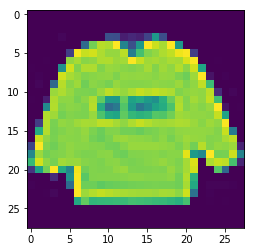
\includegraphics{output_10_0.jpg}
    
    Напишем функции тренировки и валидации моделей на данных

    \begin{Verbatim}[commandchars=\\\{\}]
{\color{incolor}In [{\color{incolor}9}]:} \PY{k}{def} \PY{n+nf}{evaluate}\PY{p}{(}\PY{n}{model}\PY{p}{)}\PY{p}{:}
            \PY{n}{correct} \PY{o}{=} \PY{l+m+mi}{0} 
            \PY{k}{for} \PY{n}{test\PYZus{}imgs}\PY{p}{,} \PY{n}{test\PYZus{}labels} \PY{o+ow}{in} \PY{n}{test\PYZus{}loader}\PY{p}{:}
                \PY{n}{test\PYZus{}imgs} \PY{o}{=} \PY{n}{Variable}\PY{p}{(}\PY{n}{test\PYZus{}imgs}\PY{p}{)}\PY{o}{.}\PY{n}{float}\PY{p}{(}\PY{p}{)}
                
                \PY{n}{output} \PY{o}{=} \PY{n}{model}\PY{p}{(}\PY{n}{test\PYZus{}imgs}\PY{p}{)}
                \PY{n}{predicted} \PY{o}{=} \PY{n}{torch}\PY{o}{.}\PY{n}{max}\PY{p}{(}\PY{n}{output}\PY{p}{,}\PY{l+m+mi}{1}\PY{p}{)}\PY{p}{[}\PY{l+m+mi}{1}\PY{p}{]}
                \PY{n}{correct} \PY{o}{+}\PY{o}{=} \PY{p}{(}\PY{n}{predicted} \PY{o}{==} \PY{n}{test\PYZus{}labels}\PY{p}{)}\PY{o}{.}\PY{n}{sum}\PY{p}{(}\PY{p}{)}
            \PY{n+nb}{print}\PY{p}{(}\PY{l+s+s2}{\PYZdq{}}\PY{l+s+s2}{Test accuracy:}\PY{l+s+si}{\PYZob{}:.3f\PYZcb{}}\PY{l+s+s2}{\PYZpc{}}\PY{l+s+s2}{ }\PY{l+s+s2}{\PYZdq{}}\PY{o}{.}\PY{n}{format}\PY{p}{(} \PY{n+nb}{float}\PY{p}{(}\PY{n}{correct}\PY{p}{)} \PY{o}{/} \PY{p}{(}\PY{n+nb}{len}\PY{p}{(}\PY{n}{test\PYZus{}loader}\PY{p}{)}\PY{o}{*}\PY{n}{BATCH\PYZus{}SIZE}\PY{p}{)}\PY{p}{)}\PY{p}{)}
        
            
        \PY{k}{def} \PY{n+nf}{fit}\PY{p}{(}\PY{n}{model}\PY{p}{,} \PY{n}{train\PYZus{}loader}\PY{p}{,} \PY{n}{epoch\PYZus{}number}\PY{o}{=}\PY{l+m+mi}{5}\PY{p}{)}\PY{p}{:}
            \PY{n}{optimizer} \PY{o}{=} \PY{n}{torch}\PY{o}{.}\PY{n}{optim}\PY{o}{.}\PY{n}{Adam}\PY{p}{(}\PY{n}{model}\PY{o}{.}\PY{n}{parameters}\PY{p}{(}\PY{p}{)}\PY{p}{)}
            \PY{n}{error} \PY{o}{=} \PY{n}{nn}\PY{o}{.}\PY{n}{CrossEntropyLoss}\PY{p}{(}\PY{p}{)}
            \PY{n}{model}\PY{o}{.}\PY{n}{train}\PY{p}{(}\PY{p}{)}
            
            \PY{k}{for} \PY{n}{epoch} \PY{o+ow}{in} \PY{n+nb}{range}\PY{p}{(}\PY{n}{epoch\PYZus{}number}\PY{p}{)}\PY{p}{:}
                \PY{n}{correct} \PY{o}{=} \PY{l+m+mi}{0}
                
                \PY{k}{for} \PY{n}{batch\PYZus{}idx}\PY{p}{,} \PY{p}{(}\PY{n}{X\PYZus{}batch}\PY{p}{,} \PY{n}{y\PYZus{}batch}\PY{p}{)} \PY{o+ow}{in} \PY{n+nb}{enumerate}\PY{p}{(}\PY{n}{train\PYZus{}loader}\PY{p}{)}\PY{p}{:}
                    \PY{n}{var\PYZus{}X\PYZus{}batch} \PY{o}{=} \PY{n}{Variable}\PY{p}{(}\PY{n}{X\PYZus{}batch}\PY{p}{)}\PY{o}{.}\PY{n}{float}\PY{p}{(}\PY{p}{)}
                    \PY{n}{var\PYZus{}y\PYZus{}batch} \PY{o}{=} \PY{n}{Variable}\PY{p}{(}\PY{n}{y\PYZus{}batch}\PY{p}{)}
                    
                    \PY{n}{optimizer}\PY{o}{.}\PY{n}{zero\PYZus{}grad}\PY{p}{(}\PY{p}{)}
                    \PY{n}{output} \PY{o}{=} \PY{n}{model}\PY{p}{(}\PY{n}{var\PYZus{}X\PYZus{}batch}\PY{p}{)}
                    \PY{n}{loss} \PY{o}{=} \PY{n}{error}\PY{p}{(}\PY{n}{output}\PY{p}{,} \PY{n}{var\PYZus{}y\PYZus{}batch}\PY{p}{)}
                    \PY{n}{loss}\PY{o}{.}\PY{n}{backward}\PY{p}{(}\PY{p}{)}
                    \PY{n}{optimizer}\PY{o}{.}\PY{n}{step}\PY{p}{(}\PY{p}{)}
        
                    \PY{n}{predicted} \PY{o}{=} \PY{n}{torch}\PY{o}{.}\PY{n}{max}\PY{p}{(}\PY{n}{output}\PY{o}{.}\PY{n}{data}\PY{p}{,} \PY{l+m+mi}{1}\PY{p}{)}\PY{p}{[}\PY{l+m+mi}{1}\PY{p}{]} 
                    \PY{n}{correct} \PY{o}{+}\PY{o}{=} \PY{p}{(}\PY{n}{predicted} \PY{o}{==} \PY{n}{var\PYZus{}y\PYZus{}batch}\PY{p}{)}\PY{o}{.}\PY{n}{sum}\PY{p}{(}\PY{p}{)}
                    \PY{k}{if} \PY{n}{batch\PYZus{}idx} \PY{o}{\PYZpc{}} \PY{l+m+mi}{500} \PY{o}{==} \PY{l+m+mi}{0}\PY{p}{:}
                        \PY{n+nb}{print}\PY{p}{(}\PY{l+s+s1}{\PYZsq{}}\PY{l+s+s1}{Epoch : }\PY{l+s+si}{\PYZob{}\PYZcb{}}\PY{l+s+s1}{ [}\PY{l+s+si}{\PYZob{}\PYZcb{}}\PY{l+s+s1}{/}\PY{l+s+si}{\PYZob{}\PYZcb{}}\PY{l+s+s1}{ (}\PY{l+s+si}{\PYZob{}:.0f\PYZcb{}}\PY{l+s+s1}{\PYZpc{}}\PY{l+s+s1}{)]}\PY{l+s+se}{\PYZbs{}t}\PY{l+s+s1}{Loss: }\PY{l+s+si}{\PYZob{}:.6f\PYZcb{}}\PY{l+s+se}{\PYZbs{}t}\PY{l+s+s1}{ Accuracy:}\PY{l+s+si}{\PYZob{}:.3f\PYZcb{}}\PY{l+s+s1}{\PYZpc{}}\PY{l+s+s1}{\PYZsq{}}\PY{o}{.}\PY{n}{format}\PY{p}{(}
                            \PY{n}{epoch}\PY{p}{,} \PY{n}{batch\PYZus{}idx}\PY{o}{*}\PY{n+nb}{len}\PY{p}{(}\PY{n}{X\PYZus{}batch}\PY{p}{)}\PY{p}{,} \PY{n+nb}{len}\PY{p}{(}\PY{n}{train\PYZus{}loader}\PY{o}{.}\PY{n}{dataset}\PY{p}{)}\PY{p}{,} \PY{l+m+mf}{100.}\PY{o}{*}\PY{n}{batch\PYZus{}idx} \PY{o}{/} \PY{n+nb}{len}\PY{p}{(}\PY{n}{train\PYZus{}loader}\PY{p}{)}\PY{p}{,} \PY{n}{loss}\PY{o}{.}\PY{n}{data}\PY{p}{,} \PY{n+nb}{float}\PY{p}{(}\PY{n}{correct}\PY{o}{*}\PY{l+m+mi}{100}\PY{p}{)} \PY{o}{/} \PY{n+nb}{float}\PY{p}{(}\PY{n}{BATCH\PYZus{}SIZE}\PY{o}{*}\PY{p}{(}\PY{n}{batch\PYZus{}idx}\PY{o}{+}\PY{l+m+mi}{1}\PY{p}{)}\PY{p}{)}\PY{p}{)}\PY{p}{)}
\end{Verbatim}


    \begin{Verbatim}[commandchars=\\\{\}]
{\color{incolor}In [{\color{incolor}10}]:} \PY{o}{\PYZpc{}\PYZpc{}}\PY{k}{time}
         evaluate(bnet)
\end{Verbatim}


    \begin{Verbatim}[commandchars=\\\{\}]
Test accuracy:0.912\% 
CPU times: user 14.8 s, sys: 0 ns, total: 14.8 s
Wall time: 7.36 s

    \end{Verbatim}

    Основная задача - дистрилировать знания из этой модели в более
компактную модель.

Архитектура маленькой модели представлена ниже. Мы возьмем сеть с двумя
полносвязанными слоями с 20 нейронами: 139-20, 20-10

    \begin{Verbatim}[commandchars=\\\{\}]
{\color{incolor}In [{\color{incolor}11}]:} \PY{k}{class} \PY{n+nc}{SmallConvNet}\PY{p}{(}\PY{n}{nn}\PY{o}{.}\PY{n}{Module}\PY{p}{)}\PY{p}{:}
             \PY{k}{def} \PY{n+nf}{\PYZus{}\PYZus{}init\PYZus{}\PYZus{}}\PY{p}{(}\PY{n+nb+bp}{self}\PY{p}{)}\PY{p}{:}
                 \PY{n+nb}{super}\PY{p}{(}\PY{n}{SmallConvNet}\PY{p}{,} \PY{n+nb+bp}{self}\PY{p}{)}\PY{o}{.}\PY{n+nf+fm}{\PYZus{}\PYZus{}init\PYZus{}\PYZus{}}\PY{p}{(}\PY{p}{)}
                 \PY{n+nb+bp}{self}\PY{o}{.}\PY{n}{conv1} \PY{o}{=} \PY{n}{nn}\PY{o}{.}\PY{n}{Conv2d}\PY{p}{(}\PY{l+m+mi}{1}\PY{p}{,} \PY{l+m+mi}{1}\PY{p}{,} \PY{l+m+mi}{3}\PY{p}{)}
                 \PY{n+nb+bp}{self}\PY{o}{.}\PY{n}{fc1} \PY{o}{=} \PY{n}{nn}\PY{o}{.}\PY{n}{Linear}\PY{p}{(}\PY{l+m+mi}{1} \PY{o}{*} \PY{l+m+mi}{13} \PY{o}{*} \PY{l+m+mi}{13}\PY{p}{,} \PY{l+m+mi}{20}\PY{p}{)}
                 \PY{n+nb+bp}{self}\PY{o}{.}\PY{n}{fc3} \PY{o}{=} \PY{n}{nn}\PY{o}{.}\PY{n}{Linear}\PY{p}{(}\PY{l+m+mi}{20}\PY{p}{,} \PY{l+m+mi}{10}\PY{p}{)}
         
             \PY{k}{def} \PY{n+nf}{forward}\PY{p}{(}\PY{n+nb+bp}{self}\PY{p}{,} \PY{n}{x}\PY{p}{)}\PY{p}{:}
                 \PY{n}{x} \PY{o}{=} \PY{n}{F}\PY{o}{.}\PY{n}{max\PYZus{}pool2d}\PY{p}{(}\PY{n}{F}\PY{o}{.}\PY{n}{relu}\PY{p}{(}\PY{n+nb+bp}{self}\PY{o}{.}\PY{n}{conv1}\PY{p}{(}\PY{n}{x}\PY{p}{)}\PY{p}{)}\PY{p}{,} \PY{l+m+mi}{2}\PY{p}{)}
                 \PY{n}{x} \PY{o}{=} \PY{n}{x}\PY{o}{.}\PY{n}{view}\PY{p}{(}\PY{o}{\PYZhy{}}\PY{l+m+mi}{1}\PY{p}{,} \PY{n+nb+bp}{self}\PY{o}{.}\PY{n}{num\PYZus{}flat\PYZus{}features}\PY{p}{(}\PY{n}{x}\PY{p}{)}\PY{p}{)}
                 \PY{n}{x} \PY{o}{=} \PY{n}{F}\PY{o}{.}\PY{n}{relu}\PY{p}{(}\PY{n+nb+bp}{self}\PY{o}{.}\PY{n}{fc1}\PY{p}{(}\PY{n}{x}\PY{p}{)}\PY{p}{)}
                 \PY{n}{x} \PY{o}{=} \PY{n+nb+bp}{self}\PY{o}{.}\PY{n}{fc3}\PY{p}{(}\PY{n}{x}\PY{p}{)}
                 \PY{k}{return} \PY{n}{x}
         
             \PY{k}{def} \PY{n+nf}{num\PYZus{}flat\PYZus{}features}\PY{p}{(}\PY{n+nb+bp}{self}\PY{p}{,} \PY{n}{x}\PY{p}{)}\PY{p}{:}
                 \PY{n}{size} \PY{o}{=} \PY{n}{x}\PY{o}{.}\PY{n}{size}\PY{p}{(}\PY{p}{)}\PY{p}{[}\PY{l+m+mi}{1}\PY{p}{:}\PY{p}{]}
                 \PY{n}{num\PYZus{}features} \PY{o}{=} \PY{l+m+mi}{1}
                 \PY{k}{for} \PY{n}{s} \PY{o+ow}{in} \PY{n}{size}\PY{p}{:}
                     \PY{n}{num\PYZus{}features} \PY{o}{*}\PY{o}{=} \PY{n}{s}
                 \PY{k}{return} \PY{n}{num\PYZus{}features}
\end{Verbatim}


    Объявим простую функцию для подсчета количества параметров

    \begin{Verbatim}[commandchars=\\\{\}]
{\color{incolor}In [{\color{incolor}12}]:} \PY{k}{def} \PY{n+nf}{calc\PYZus{}weights}\PY{p}{(}\PY{n}{model}\PY{p}{)}\PY{p}{:}
             \PY{n}{result} \PY{o}{=} \PY{l+m+mi}{0}
             \PY{k}{for} \PY{n}{layer} \PY{o+ow}{in} \PY{n}{model}\PY{o}{.}\PY{n}{children}\PY{p}{(}\PY{p}{)}\PY{p}{:}
                 \PY{k}{if} \PY{n+nb}{hasattr}\PY{p}{(}\PY{n}{layer}\PY{p}{,} \PY{l+s+s1}{\PYZsq{}}\PY{l+s+s1}{weight}\PY{l+s+s1}{\PYZsq{}}\PY{p}{)}\PY{p}{:}
                     \PY{n}{result} \PY{o}{+}\PY{o}{=} \PY{n+nb}{len}\PY{p}{(}\PY{n}{layer}\PY{o}{.}\PY{n}{weight}\PY{o}{.}\PY{n}{reshape}\PY{p}{(}\PY{o}{\PYZhy{}}\PY{l+m+mi}{1}\PY{p}{)}\PY{p}{)}
             \PY{k}{return} \PY{n}{result}
\end{Verbatim}


    \begin{Verbatim}[commandchars=\\\{\}]
{\color{incolor}In [{\color{incolor}13}]:} \PY{n}{scnet} \PY{o}{=} \PY{n}{SmallConvNet}\PY{p}{(}\PY{p}{)}
\end{Verbatim}


    \begin{Verbatim}[commandchars=\\\{\}]
{\color{incolor}In [{\color{incolor}14}]:} \PY{n}{calc\PYZus{}weights}\PY{p}{(}\PY{n}{scnet}\PY{p}{)}
\end{Verbatim}


\begin{Verbatim}[commandchars=\\\{\}]
{\color{outcolor}Out[{\color{outcolor}14}]:} 3589
\end{Verbatim}
            
    \begin{Verbatim}[commandchars=\\\{\}]
{\color{incolor}In [{\color{incolor}15}]:} \PY{o}{\PYZpc{}\PYZpc{}}\PY{k}{time}
         evaluate(scnet)
\end{Verbatim}


    \begin{Verbatim}[commandchars=\\\{\}]
Test accuracy:0.069\% 
CPU times: user 5.62 s, sys: 608 µs, total: 5.62 s
Wall time: 2.79 s

    \end{Verbatim}

    Видим, что модель гораздо меньше первой и имеет 3.5 тысячи параметров.
Также время инференса для нее значительно меньше, примерно в 3 раза.

Далее посмотрим, какое качество модель выдает сама по себе. Обучим ее на
данных и провалидируем.

    \begin{Verbatim}[commandchars=\\\{\}]
{\color{incolor}In [{\color{incolor}16}]:} \PY{n}{torch}\PY{o}{.}\PY{n}{manual\PYZus{}seed}\PY{p}{(}\PY{n}{SEED}\PY{p}{)}
         \PY{n}{fit}\PY{p}{(}\PY{n}{scnet}\PY{p}{,} \PY{n}{train\PYZus{}loader}\PY{p}{)}
\end{Verbatim}


    \begin{Verbatim}[commandchars=\\\{\}]
Epoch : 0 [0/60000]	Loss: 25.429 Accuracy:9.375\%
Epoch : 0 [16000/60000]	Loss: 1.014 Accuracy:48.235\%
Epoch : 0 [32000/60000]	Loss: 0.753 Accuracy:57.752\%
Epoch : 0 [48000/60000]	Loss: 1.053 Accuracy:61.882\%
Epoch : 1 [0/60000]	Loss: 0.88 Accuracy:68.750\%
Epoch : 1 [16000/60000]	Loss: 0.659 Accuracy:73.478\%
Epoch : 1 [32000/60000]	Loss: 0.695 Accuracy:74.294\%
Epoch : 1 [48000/60000]	Loss: 0.873 Accuracy:75.117\%
Epoch : 2 [0/60000]	Loss: 0.707 Accuracy:68.750\%
Epoch : 2 [16000/60000]	Loss: 0.552 Accuracy:77.813\%
Epoch : 2 [32000/60000]	Loss: 0.583 Accuracy:78.038\%
Epoch : 2 [48000/60000]	Loss: 0.785 Accuracy:78.543\%
Epoch : 3 [0/60000]	Loss: 0.688 Accuracy:68.750\%
Epoch : 3 [16000/60000]	Loss: 0.44  Accuracy:80.252\%
Epoch : 3 [32000/60000]	Loss: 0.528 Accuracy:80.313\%
Epoch : 3 [48000/60000]	Loss: 0.763 Accuracy:80.590\%
Epoch : 4 [0/60000]	Loss: 0.625 Accuracy:78.125\%
Epoch : 4 [16000/60000]	Loss: 0.391 Accuracy:81.437\%
Epoch : 4 [32000/60000]	Loss: 0.547 Accuracy:81.559\%
Epoch : 4 [48000/60000]	Loss: 0.764 Accuracy:81.666\%

    \end{Verbatim}

    \begin{Verbatim}[commandchars=\\\{\}]
{\color{incolor}In [{\color{incolor}17}]:} \PY{n}{evaluate}\PY{p}{(}\PY{n}{scnet}\PY{p}{)}
\end{Verbatim}


    \begin{Verbatim}[commandchars=\\\{\}]
Test accuracy:0.827\% 

    \end{Verbatim}

    Модель сама по себе выдает \texttt{82.7\%} точности. Давайте применим
алгоритм дистиляции знаний из более крупной модели и попробуем улучшить
результат.

Мы объявим функцию Дивергенция Кульбака-Лейблера, чтобы подсчитать
кросс-энтропию между двумя распределениями. 

    \begin{Verbatim}[commandchars=\\\{\}]
{\color{incolor}In [{\color{incolor}18}]:} \PY{k}{def} \PY{n+nf}{distill}\PY{p}{(}\PY{n}{teacher\PYZus{}model}\PY{p}{,} \PY{n}{student\PYZus{}model}\PY{p}{,} \PY{n}{train\PYZus{}loader}\PY{p}{,} \PY{n}{epoch\PYZus{}number}\PY{o}{=}\PY{l+m+mi}{5}\PY{p}{,} \PY{n}{alpha}\PY{o}{=}\PY{l+m+mf}{0.7}\PY{p}{,} \PY{n}{temperature}\PY{o}{=}\PY{l+m+mi}{5}\PY{p}{)}\PY{p}{:}
             \PY{k}{def} \PY{n+nf}{error\PYZus{}and\PYZus{}output}\PY{p}{(}\PY{n}{var\PYZus{}X\PYZus{}batch}\PY{p}{,} \PY{n}{var\PYZus{}y\PYZus{}batch}\PY{p}{)}\PY{p}{:}
         
                 \PY{n}{kldloss} \PY{o}{=} \PY{n}{nn}\PY{o}{.}\PY{n}{KLDivLoss}\PY{p}{(}\PY{p}{)}  
                 \PY{n}{celoss} \PY{o}{=} \PY{n}{nn}\PY{o}{.}\PY{n}{CrossEntropyLoss}\PY{p}{(}\PY{p}{)}
                 
                 \PY{n}{teacher\PYZus{}logits} \PY{o}{=} \PY{n}{teacher\PYZus{}model}\PY{p}{(}\PY{n}{var\PYZus{}X\PYZus{}batch}\PY{p}{)}
                 \PY{n}{student\PYZus{}logits} \PY{o}{=} \PY{n}{student\PYZus{}model}\PY{p}{(}\PY{n}{var\PYZus{}X\PYZus{}batch}\PY{p}{)}
                 
                 \PY{n}{soft\PYZus{}predictions} \PY{o}{=} \PY{n}{F}\PY{o}{.}\PY{n}{log\PYZus{}softmax}\PY{p}{(} \PY{n}{student\PYZus{}logits} \PY{o}{/} \PY{n}{temperature}\PY{p}{,} \PY{n}{dim}\PY{o}{=}\PY{l+m+mi}{1} \PY{p}{)}
                 \PY{n}{soft\PYZus{}labels} \PY{o}{=} \PY{n}{F}\PY{o}{.}\PY{n}{softmax}\PY{p}{(} \PY{n}{teacher\PYZus{}logits} \PY{o}{/} \PY{n}{temperature}\PY{p}{,} \PY{n}{dim}\PY{o}{=}\PY{l+m+mi}{1} \PY{p}{)}
                 \PY{n}{distillation\PYZus{}loss} \PY{o}{=} \PY{n}{kldloss}\PY{p}{(}\PY{n}{soft\PYZus{}predictions}\PY{p}{,} \PY{n}{soft\PYZus{}labels}\PY{p}{)}
                 
                 \PY{n}{student\PYZus{}loss} \PY{o}{=} \PY{n}{celoss}\PY{p}{(}\PY{n}{student\PYZus{}logits}\PY{p}{,} \PY{n}{var\PYZus{}y\PYZus{}batch}\PY{p}{)}
                 
                 \PY{k}{return} \PY{n}{distillation\PYZus{}loss} \PY{o}{*} \PY{n}{alpha} \PY{o}{+} \PY{n}{student\PYZus{}loss} \PY{o}{*} \PY{p}{(}\PY{l+m+mi}{1} \PY{o}{\PYZhy{}} \PY{n}{alpha}\PY{p}{)}\PY{p}{,} \PY{n}{student\PYZus{}logits}
             
             \PY{n}{optimizer} \PY{o}{=} \PY{n}{torch}\PY{o}{.}\PY{n}{optim}\PY{o}{.}\PY{n}{Adam}\PY{p}{(}\PY{n}{student\PYZus{}model}\PY{o}{.}\PY{n}{parameters}\PY{p}{(}\PY{p}{)}\PY{p}{)}
             \PY{n}{student\PYZus{}model}\PY{o}{.}\PY{n}{train}\PY{p}{(}\PY{p}{)}
             
             \PY{k}{for} \PY{n}{epoch} \PY{o+ow}{in} \PY{n+nb}{range}\PY{p}{(}\PY{n}{epoch\PYZus{}number}\PY{p}{)}\PY{p}{:}
                 \PY{n}{correct} \PY{o}{=} \PY{l+m+mi}{0}
                 \PY{k}{for} \PY{n}{batch\PYZus{}idx}\PY{p}{,} \PY{p}{(}\PY{n}{X\PYZus{}batch}\PY{p}{,} \PY{n}{y\PYZus{}batch}\PY{p}{)} \PY{o+ow}{in} \PY{n+nb}{enumerate}\PY{p}{(}\PY{n}{train\PYZus{}loader}\PY{p}{)}\PY{p}{:}
                     
                     \PY{n}{var\PYZus{}X\PYZus{}batch} \PY{o}{=} \PY{n}{Variable}\PY{p}{(}\PY{n}{X\PYZus{}batch}\PY{p}{)}\PY{o}{.}\PY{n}{float}\PY{p}{(}\PY{p}{)}
                     \PY{n}{var\PYZus{}y\PYZus{}batch} \PY{o}{=} \PY{n}{Variable}\PY{p}{(}\PY{n}{y\PYZus{}batch}\PY{p}{)}
                     \PY{n}{optimizer}\PY{o}{.}\PY{n}{zero\PYZus{}grad}\PY{p}{(}\PY{p}{)}
                     \PY{n}{loss}\PY{p}{,} \PY{n}{output} \PY{o}{=} \PY{n}{error\PYZus{}and\PYZus{}output}\PY{p}{(}\PY{n}{var\PYZus{}X\PYZus{}batch}\PY{p}{,} \PY{n}{var\PYZus{}y\PYZus{}batch}\PY{p}{)}
                     \PY{n}{loss}\PY{o}{.}\PY{n}{backward}\PY{p}{(}\PY{p}{)}
                     \PY{n}{optimizer}\PY{o}{.}\PY{n}{step}\PY{p}{(}\PY{p}{)}
         
                     \PY{n}{predicted} \PY{o}{=} \PY{n}{torch}\PY{o}{.}\PY{n}{max}\PY{p}{(}\PY{n}{output}\PY{o}{.}\PY{n}{data}\PY{p}{,} \PY{l+m+mi}{1}\PY{p}{)}\PY{p}{[}\PY{l+m+mi}{1}\PY{p}{]} 
                     \PY{n}{correct} \PY{o}{+}\PY{o}{=} \PY{p}{(}\PY{n}{predicted} \PY{o}{==} \PY{n}{var\PYZus{}y\PYZus{}batch}\PY{p}{)}\PY{o}{.}\PY{n}{sum}\PY{p}{(}\PY{p}{)}
                     \PY{k}{if} \PY{n}{batch\PYZus{}idx} \PY{o}{\PYZpc{}} \PY{l+m+mi}{200} \PY{o}{==} \PY{l+m+mi}{0}\PY{p}{:}
                         \PY{n+nb}{print}\PY{p}{(}\PY{l+s+s1}{\PYZsq{}}\PY{l+s+s1}{Epoch : }\PY{l+s+si}{\PYZob{}\PYZcb{}}\PY{l+s+s1}{ [}\PY{l+s+si}{\PYZob{}\PYZcb{}}\PY{l+s+s1}{/}\PY{l+s+si}{\PYZob{}\PYZcb{}}\PY{l+s+s1}{ (}\PY{l+s+si}{\PYZob{}:.0f\PYZcb{}}\PY{l+s+s1}{\PYZpc{}}\PY{l+s+s1}{)]}\PY{l+s+se}{\PYZbs{}t}\PY{l+s+s1}{Loss: }\PY{l+s+si}{\PYZob{}:.6f\PYZcb{}}\PY{l+s+se}{\PYZbs{}t}\PY{l+s+s1}{ Accuracy:}\PY{l+s+si}{\PYZob{}:.3f\PYZcb{}}\PY{l+s+s1}{\PYZpc{}}\PY{l+s+s1}{\PYZsq{}}\PY{o}{.}\PY{n}{format}\PY{p}{(}
                             \PY{n}{epoch}\PY{p}{,} \PY{n}{batch\PYZus{}idx}\PY{o}{*}\PY{n+nb}{len}\PY{p}{(}\PY{n}{X\PYZus{}batch}\PY{p}{)}\PY{p}{,} \PY{n+nb}{len}\PY{p}{(}\PY{n}{train\PYZus{}loader}\PY{o}{.}\PY{n}{dataset}\PY{p}{)}\PY{p}{,} \PY{l+m+mf}{100.}\PY{o}{*}\PY{n}{batch\PYZus{}idx} \PY{o}{/} \PY{n+nb}{len}\PY{p}{(}\PY{n}{train\PYZus{}loader}\PY{p}{)}\PY{p}{,} \PY{n}{loss}\PY{o}{.}\PY{n}{data}\PY{p}{,} \PY{n+nb}{float}\PY{p}{(}\PY{n}{correct}\PY{o}{*}\PY{l+m+mi}{100}\PY{p}{)} \PY{o}{/} \PY{n+nb}{float}\PY{p}{(}\PY{n}{BATCH\PYZus{}SIZE}\PY{o}{*}\PY{p}{(}\PY{n}{batch\PYZus{}idx}\PY{o}{+}\PY{l+m+mi}{1}\PY{p}{)}\PY{p}{)}\PY{p}{)}\PY{p}{)}
\end{Verbatim}


    Обучим нашу сеть-ученика, пользуясь знаниями сети-учителя

    \begin{Verbatim}[commandchars=\\\{\}]
{\color{incolor}In [{\color{incolor}21}]:} \PY{n}{distill}\PY{p}{(}\PY{n}{bnet}\PY{p}{,} \PY{n}{scnet}\PY{p}{,} \PY{n}{train\PYZus{}loader}\PY{p}{,} \PY{n}{epoch\PYZus{}number}\PY{o}{=}\PY{l+m+mi}{5}\PY{p}{,} \PY{n}{temperature}\PY{o}{=}\PY{l+m+mf}{5.0}\PY{p}{,} \PY{n}{alpha}\PY{o}{=}\PY{l+m+mf}{0.7}\PY{p}{)}
\end{Verbatim}


    \begin{Verbatim}[commandchars=\\\{\}]
Epoch : 0 [0/60000]	Loss: 0.168 Accuracy:81.250\%
Epoch : 0 [6400/60000]	Loss: 0.173	Accuracy:82.743\%
Epoch : 0 [12800/60000]	Loss: 0.259 Accuracy:82.403\%
Epoch : 0 [19200/60000]	Loss: 0.155 Accuracy:82.607\%
Epoch : 0 [25600/60000]	Loss: 0.129 Accuracy:82.557\%
Epoch : 0 [32000/60000]	Loss: 0.177 Accuracy:82.549\%
Epoch : 0 [38400/60000]	Loss: 0.159 Accuracy:82.639\%
Epoch : 0 [44800/60000]	Loss: 0.149 Accuracy:82.780\%
Epoch : 0 [51200/60000]	Loss: 0.115 Accuracy:82.749\%
Epoch : 0 [57600/60000]	Loss: 0.114 Accuracy:82.711\%
Epoch : 1 [0/60000]	Loss: 0.167 Accuracy:81.250\%
Epoch : 1 [6400/60000]	Loss: 0.175 Accuracy:83.364\%
Epoch : 1 [12800/60000]	Loss: 0.246 Accuracy:82.949\%
Epoch : 1 [19200/60000]	Loss: 0.161 Accuracy:83.023\%
Epoch : 1 [25600/60000]	Loss: 0.123 Accuracy:83.033\%
Epoch : 1 [32000/60000]	Loss: 0.192 Accuracy:82.936\%
Epoch : 1 [38400/60000]	Loss: 0.156 Accuracy:82.999\%
Epoch : 1 [51200/60000]	Loss: 0.113 Accuracy:83.102\%
Epoch : 1 [57600/60000]	Loss: 0.111 Accuracy:83.055\%
Epoch : 2 [0/60000]	Loss: 0.166 Accuracy:84.375\%
Epoch : 2 [6400/60000]	Loss: 0.171 Accuracy:83.567\%
Epoch : 2 [12800/60000]	Loss: 0.244 Accuracy:83.229\%
Epoch : 2 [19200/60000]	Loss: 0.142 Accuracy:83.325\%
Epoch : 2 [25600/60000]	Loss: 0.119 Accuracy:83.263\%
Epoch : 2 [32000/60000]	Loss: 0.186 Accuracy:83.232\%
Epoch : 2 [38400/60000]	Loss: 0.160 Accuracy:83.287\%
Epoch : 2 [44800/60000]	Loss: 0.150 Accuracy:83.427\%
Epoch : 2 [51200/60000]	Loss: 0.108 Accuracy:83.434\%
Epoch : 2 [57600/60000]	Loss: 0.114 Accuracy:83.362\%
Epoch : 3 [0/60000]	Loss: 0.17 Accuracy:81.250\%
Epoch : 3 [6400/60000]	Loss: 0.173 Accuracy:83.800\%
Epoch : 3 [12800/60000]	Loss: 0.24 Accuracy:83.409\%
Epoch : 3 [19200/60000]	Loss: 0.135 Accuracy:83.475\%
Epoch : 3 [25600/60000]	Loss: 0.116 Accuracy:83.446\%
Epoch : 3 [38400/60000]	Loss: 0.157 Accuracy:83.516\%
Epoch : 3 [44800/60000]	Loss: 0.152 Accuracy:83.632\%
Epoch : 3 [51200/60000]	Loss: 0.114 Accuracy:83.627\%
Epoch : 3 [57600/60000]	Loss: 0.107 Accuracy:83.577\%
Epoch : 4 [0/60000]	Loss: 0.172 Accuracy:81.250\%
Epoch : 4 [6400/60000]	Loss: 0.169 Accuracy:84.017\%
Epoch : 4 [12800/60000]	Loss: 0.237 Accuracy:83.814\%
Epoch : 4 [19200/60000]	Loss: 0.134 Accuracy:83.803\%
Epoch : 4 [25600/60000]	Loss: 0.118 Accuracy:83.673\%
Epoch : 4 [32000/60000]	Loss: 0.189  Accuracy:83.707\%
Epoch : 4 [44800/60000]	Loss: 0.148 Accuracy:83.920\%
Epoch : 4 [51200/60000]	Loss: 0.121 Accuracy:83.920\%
Epoch : 4 [57600/60000]	Loss: 0.103  Accuracy:83.874\%

    \end{Verbatim}

    \begin{Verbatim}[commandchars=\\\{\}]
{\color{incolor}In [{\color{incolor}22}]:} \PY{n}{evaluate}\PY{p}{(}\PY{n}{scnet}\PY{p}{)}
\end{Verbatim}


    \begin{Verbatim}[commandchars=\\\{\}]
Test accuracy:0.841\% 

    \end{Verbatim}

    Видим, что применяя дистилляцию знаний, нам удалось повысить качество
маленькой модели на несколько процентов, при этом сохранив ее
компактность.

    
\end{document}
